\documentclass{scrartcl}
\usepackage{lipsum}
%%\usepackage[french]{babel}
%%\usepackage[ngerman]{babel}


%% Choose default font for the document
%% Warning : only ONE of the following should be enabled
\usepackage{kpfonts}
%%\usepackage{libertine}

%% The following chose the default language for the document and
%% use the default typography rules for the choosen language.
\usepackage{polyglossia}
\setdefaultlanguage{english}
%% \setdefaultlanguage{german}
%%\setdefaultlanguage{french}

\usepackage[backend=biber, style=ieee]{biblatex}
\addbibresource{template.bib}

\usepackage{graphicx}
\graphicspath{ {./im_ressources/} }


\begin{document}
\title{Visualization of a robotic arms working area}
\date{\today}   %% or \date{01 november 2018}
\author{Flückiger Quentin (\texttt{flucq1@bfh.ch}) }

\clearpage
\maketitle
\tableofcontents
\begin{enumerate}
  \item Introduction
  \item Project requirements
  \begin{itemize}
    \item Vision
    \item Goals
    \item System context
    \item Legend and additional information
    \item Table
    \item Description
    \item Stakeholder descriptions
  \end{itemize}
  \item Phase 1
  \begin{itemize}
    \item Environment setup / Modeling
    \item Animating
  \end{itemize}
  \item Voxel world
  \begin{itemize}
    \item Set up
    \item Collision
    \item Prediction
    \item Cleaning
    \item Optimization
  \end{itemize}
  \item Conclusion and future work
\end{enumerate}

\clearpage

\section{Introduction}

Work, this activity most of us must do daily to earn a salary and get on with our lives and hobbies.
During this activity we will have to deal and work with co-worker, we start to understand how people behave at our workplace 
and even maybe in general for this sort of work. The more we get used to the way our co-workers work,
and they get used to how we work, the more we can predict what will be there actions and so anticipate them to be more efficient.
But with the appearance of robot, taking more and more subtasks, it started to be difficult to predict their action 
as they have a complete different perception as we do, if we can call it perception. 
And with every update their behaviour would vary so our time getting used to them would go to waste and we would start over. 

Let’s take for example a robot on a montage chain taking a piece “A” to put it on the chain, and a human employee in front of it. 
This robot does the same pathing with its arm for weeks, but on a Monday morning after an update it has a new pattern. 
Unfortunately, the employee is unaware of this. He lets his glasses slip close to the robot, lucky him they are on the side where the robot never goes, 
so he reaches out his hand to grab them. And at this time the robot used one of the new pattern he was just improved with in the new update. 
Wouldn’t it be great to have a way to visualize and predict the movement of such a robot?

Well this project will cover the topics movements visualization of a robotic arm and prediction about its whereabout. 


\clearpage

\section{Project requirements}
\subsection{Vision}
\subsection{Goals}
\subsection{System context}
\subsection{Legend and additional information}
\subsection{Table}
\subsection{Description}
\subsection{Stakeholder descriptions}

\clearpage

\section{Phase 1}
\subsection{Environment setup / Modelling}

In the first step of phase one came all the setup of the different software, API, 
system and models to be used during the rest of the project. I decided to use Unity to develop the application for the following reasons.
I am already a little bit familiar with it, it is cross platform, the documentation is abundant, 
and it is rather easy and intuitive to take in hand. As the use of GitLab was suggested by Mr. Fuhrer 
I went with this solution to share my work and progress. But for Git to recognize the change in Unity 
files we need a special .gitignore. This .gitignore can be added when we create a repository with GitHub, 
so I decided to create the repository with GitHub and mirror it on GitLab. For this to work, we need to do 
change two settings in Unity editor settings. A step by step guide on how to setup github with unity 
can be found here https://www.studica.com/blog/how-to-setup-github-with-unity-step-by-step-instructions . 
The use of LaTex was strongly recommended as well, as it allows to see exactly what has been change in the documentation file, 
contrary to a word file for example which will erase the old one and push the new one every time a commit is done. 
To be able to use LaTex I had to instal Visual Studio Code, LaTex Compiler and Texlive. 
I had to solve a little issue where I was trying to compile with pdfTex when I had LuaLaTex. 
Afterward I looked for a free, open source 3D model of a Kuka arm robot. I came up with three solutions.

\begin{center}
  \begin{tabular}{c c c}
    1 & 2 & 3 \\
    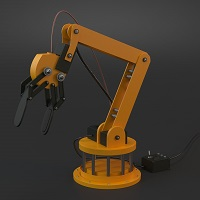
\includegraphics{industrial_robotic_arm} & 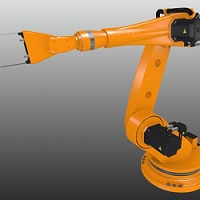
\includegraphics{kuka} & 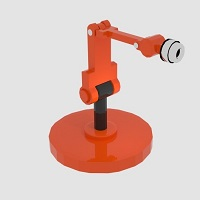
\includegraphics{robotarm_cylinder}
  \end{tabular}
\end{center}
I chose the number 2 as it was already rigged and therefore the easiest to animate at this stage. 
Before I could animate the 3D model, I decided to “purify” it as there was a lot of useless part, such as screw, bolt, cylinder. 
Doing so I reduced the size of the 3D model file by approximately the half. I used Blender to view and modify the file.

\subsection{Animating}

Once all the Software, model setup was done I could start to animate the model. To do so I used once more Blender, 
this time to animate the model we refined. I managed to do a few animations after a long try out, 
and suddenly a part of the arm was a few pixels away from the location it should be. This occurred on every animation and even the base refined model. 
I had to revert all changes done to the model, so all the animations were lost. I looked for another solution rather than continuing with Blender 
and maybe having the same issue again later. I chose to use Unity’s built in animator as a solution. 
It worked way better than I expected, was faster to develop than with Blender as well. I created a set of three times four different animations 
which pick up or drop an imaginary object on the ground, in mid-air or high in the air. 
Each one of those set is composed by one animation which turns to 90° then come back, one which turns to 180° and the two others are the same but in negative (-90°, -180°). 
I added all 12 animations to an animator which is linked to the Kuka model. This animator is a state machine, it starts in the Idle state. 
To make it play different animation (state) we change the value of an integer parameter (AnimParam) with different values 
which correspond to transition reference to one special animation. When an animation is finished playing it sets the value of the parameter to 0, 
which is the value of the Idle state, so the animator is ready to play another animation. 

To play an animation I decided to add a listener which catch if the space key is pressed and then play a random animation using UnityEngine.Random.
\begin{center}
  randomIndex = UnityEngine.Random.Range(0, totalNumberOfAnimation); 
\end{center}

The second option to play an animation is a more visual one, it allows the user to choose the amount of animations he wants to play. 
It can be chosen with a slider at runtime and then proceeded by clicking a button bellow the slider. 
This will add random integer, using the same UnityEngine.Random as before, to a stack. This stack will be used as a “playlist” to play one animation after another. 
However, I encountered a problem in which the AnimParam wasn’t set to 0 after an animation was over. 
Which leads to not being able to play any other animation or repeating the same one over and over again. 
So far, the proof led me to think it was a frame problem, so I used a frame counter as a “forced break” after every animation so the AnimParam get properly set to 0. 
This works, but now sometime the animation queue just stops playing. As a solution I thought about doing this with a coroutine.


\clearpage

\section{Voxel world}
\subsection{Set up}
\subsection{Collision}
\subsection{Prediction}
\subsection{Cleaning}
\subsection{Optimization}


\clearpage

\section{Conclusion and future work}
To be filled later


%% Print the bibibliography and add the section to the table of content
\printbibliography[heading=bibintoc]

\end{document}
